\documentclass[border=16pt,tikz]{standalone}
\usepackage{tikz}
\usetikzlibrary{positioning,arrows.meta,fit,backgrounds,calc}

\definecolor{cext}{RGB}{232,232,232}
\definecolor{cprx}{RGB}{173,216,230}
\definecolor{capp}{RGB}{144,238,144}
\definecolor{cdb} {RGB}{255,228,181}
\definecolor{cphi}{RGB}{255,175,175}
\definecolor{csec}{RGB}{255,192,203}
\definecolor{cobs}{RGB}{216,191,216}

\tikzset{
  nd/.style={draw, rounded corners=5pt,
             minimum width=2.8cm, minimum height=0.9cm,
             font=\small\sffamily, align=center, inner sep=4pt},
  ext/.style={nd, fill=cext,  draw=gray!70},
  prx/.style={nd, fill=cprx,  draw=blue!60},
  app/.style={nd, fill=capp,  draw=green!60!black},
  dbs/.style={nd, fill=cdb,   draw=orange!70},
  phi/.style={nd, fill=cphi,  draw=red!70, line width=1.2pt},
  sec/.style={nd, fill=csec,  draw=red!50},
  obs/.style={nd, fill=cobs,  draw=purple!60},
  arr/.style={-{Stealth[length=6pt,width=5pt]}, semithick, gray!60},
  darr/.style={arr, dashed, gray!50},
  grp/.style={draw, rounded corners=8pt, inner sep=8pt},
}

\begin{document}
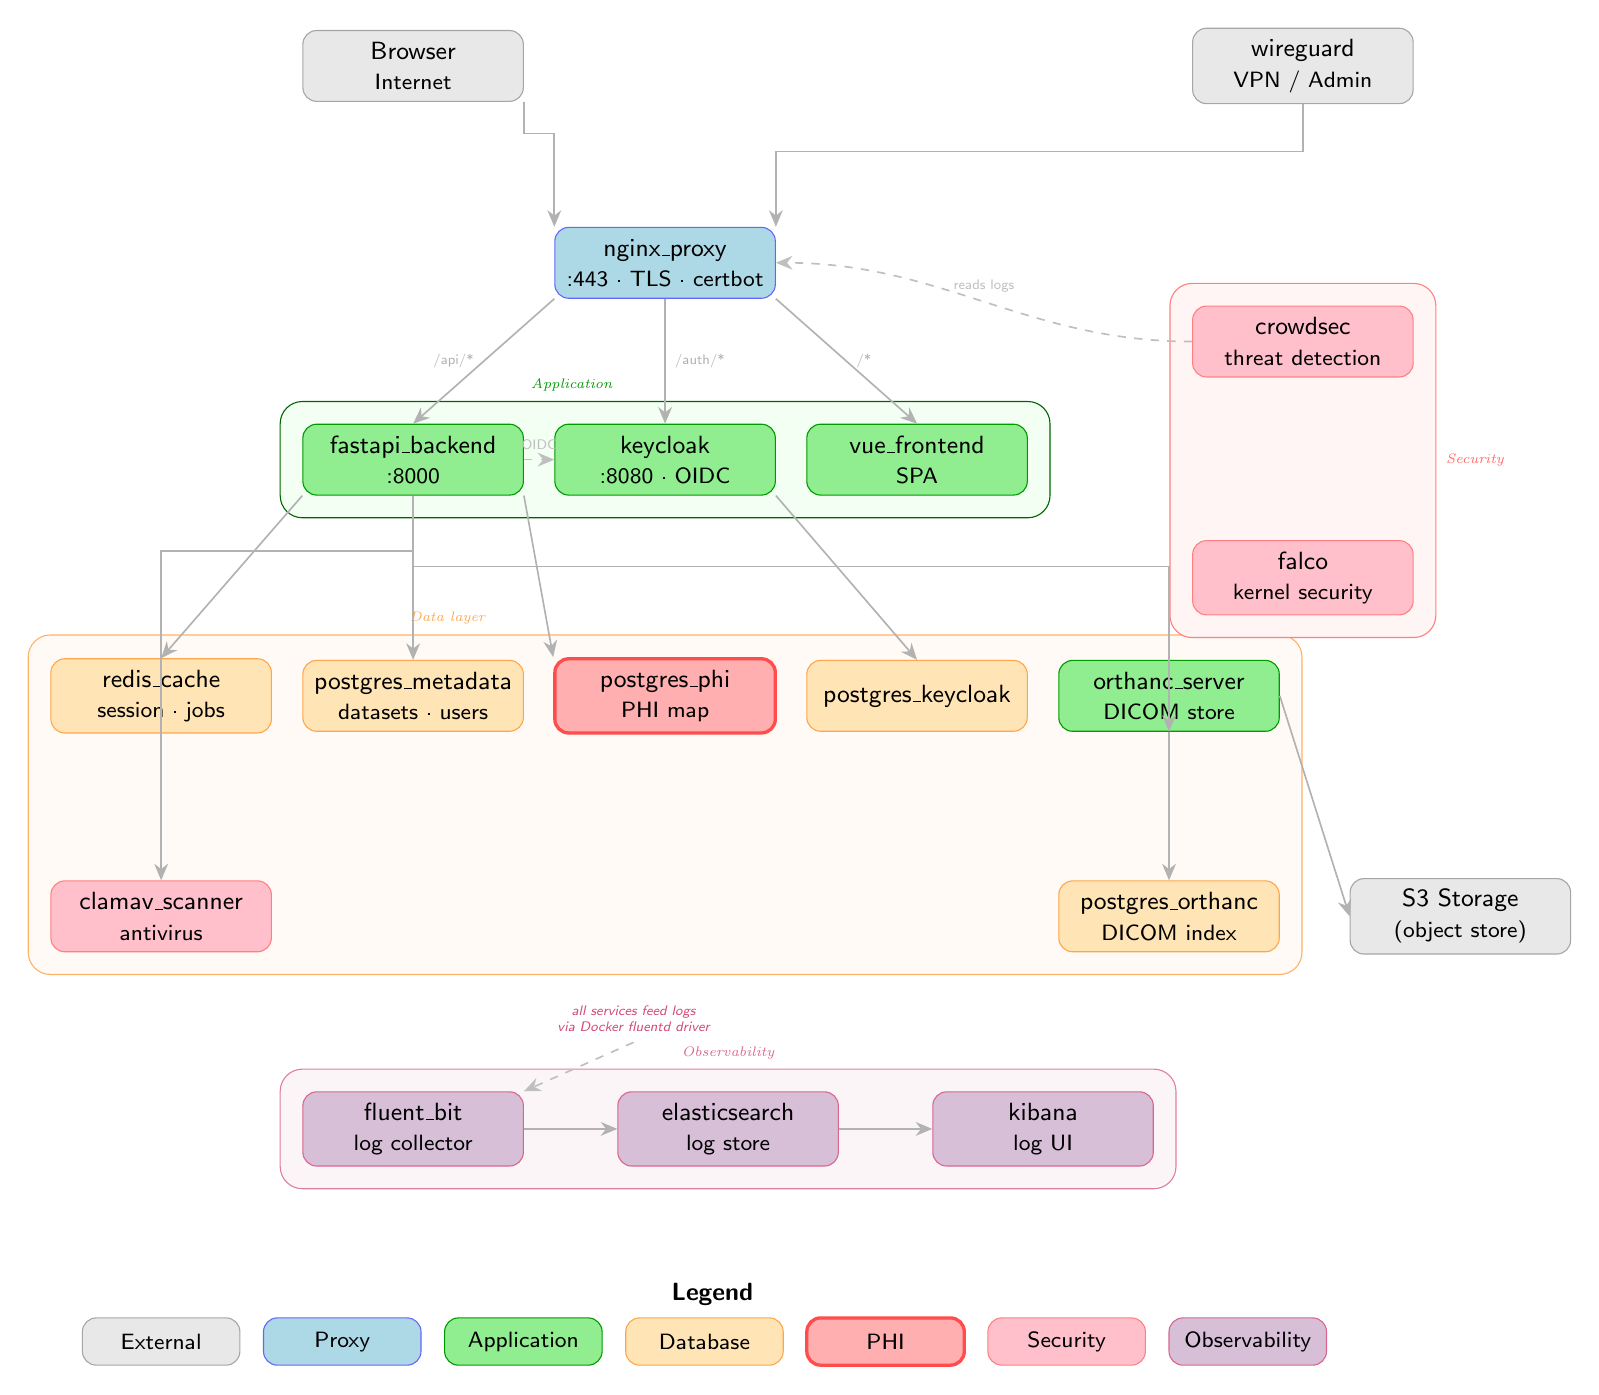
\begin{tikzpicture}

%% ---- ROW 0: External ----------------------------------------
\node[ext] (browser)   at ( 3.2,  0.0) {Browser\\{\footnotesize Internet}};
\node[ext] (wireguard) at (14.5,  0.0) {wireguard\\{\footnotesize VPN / Admin}};

%% ---- ROW 1: Edge  -------------------------------------------
\node[prx] (nginx) at (6.4, -2.5)
  {nginx\_proxy\\{\footnotesize :443 · TLS · certbot}};

%% ---- ROW 2: Application  ------------------------------------
\node[app] (fastapi)  at (3.2,  -5.0) {fastapi\_backend\\{\footnotesize :8000}};
\node[app] (keycloak) at (6.4,  -5.0) {keycloak\\{\footnotesize :8080 · OIDC}};
\node[app] (vue)      at (9.6,  -5.0) {vue\_frontend\\{\footnotesize SPA}};

%% ---- ROW 3: Data layer  -------------------------------------
\node[dbs] (redis)   at ( 0.0, -8.0) {redis\_cache\\{\footnotesize session · jobs}};
\node[dbs] (pgmeta)  at ( 3.2, -8.0) {postgres\_metadata\\{\footnotesize datasets · users}};
\node[phi] (pgphi)   at ( 6.4, -8.0) {postgres\_phi\\{\footnotesize PHI map}};
\node[dbs] (pgkc)    at ( 9.6, -8.0) {postgres\_keycloak};
\node[app] (orthanc) at (12.8, -8.0) {orthanc\_server\\{\footnotesize DICOM store}};

%% ---- ROW 4: Storage  ----------------------------------------
\node[sec] (clamav)    at ( 0.0, -10.8) {clamav\_scanner\\{\footnotesize antivirus}};
\node[dbs] (pgorthanc) at (12.8, -10.8) {postgres\_orthanc\\{\footnotesize DICOM index}};
\node[ext] (s3)        at (16.5, -10.8) {S3 Storage\\{\footnotesize (object store)}};

%% ---- SECURITY (right column)  -------------------------------
\node[sec] (crowdsec) at (14.5, -3.5) {crowdsec\\{\footnotesize threat detection}};
\node[sec] (falco)    at (14.5, -6.5) {falco\\{\footnotesize kernel security}};

%% ---- OBSERVABILITY (bottom)  --------------------------------
\node[obs] (fluentbit) at ( 3.2, -13.5) {fluent\_bit\\{\footnotesize log collector}};
\node[obs] (elastic)   at ( 7.2, -13.5) {elasticsearch\\{\footnotesize log store}};
\node[obs] (kibana)    at (11.2, -13.5) {kibana\\{\footnotesize log UI}};

%% ==== ARROWS =================================================

%% External → nginx
\draw[arr] (browser.south east) -- ++(0,-0.4) -| (nginx.north west);
\draw[arr] (wireguard.south) -- ++(0,-0.6) -| (nginx.north east);

%% nginx → apps
\draw[arr] (nginx.south west) -- node[left,  font=\tiny\sffamily]{/api/*}  (fastapi.north);
\draw[arr] (nginx.south)      -- node[right, font=\tiny\sffamily]{/auth/*} (keycloak.north);
\draw[arr] (nginx.south east) -- node[right, font=\tiny\sffamily]{/*}      (vue.north);

%% FastAPI → data layer
\draw[arr] (fastapi.south west) -- (redis.north);
\draw[arr] (fastapi.south)      -- (pgmeta.north);
\draw[arr] (fastapi.south east) -- (pgphi.north west);

%% FastAPI → ClamAV (routed left below data row)
\draw[arr] (fastapi.south) -- ++(0,-0.7) -- ++(-3.2,0) -- (clamav.north);

%% FastAPI → Orthanc (routed below application row, above data row)
\draw[arr] (fastapi.south) -- ++(0,-0.9) -| (orthanc.south);

%% FastAPI ↔ Keycloak (OIDC token verify, dashed)
\draw[darr] (fastapi.east) -- node[above, font=\tiny\sffamily]{OIDC} (keycloak.west);

%% Keycloak → postgres_keycloak
\draw[arr] (keycloak.south east) -- (pgkc.north);

%% Orthanc → storage
\draw[arr] (orthanc.south)  -- (pgorthanc.north);
\draw[arr] (orthanc.east)   -- (s3.west);

%% CrowdSec reads nginx logs
\draw[darr] (crowdsec.west) to[out=180,in=0]
  node[above, font=\tiny\sffamily]{reads logs} (nginx.east);

%% Observability chain
\draw[arr] (fluentbit) -- (elastic);
\draw[arr] (elastic)   -- (kibana);

%% Logging note (all services → fluent_bit via Docker logging driver)
\node[font=\tiny\sffamily\itshape, text=purple!70, align=center]
  at (6.0, -12.1) {all services feed logs\\via Docker fluentd driver};
\draw[darr] (6.0,-12.4) -- (fluentbit.north east);

%% ==== BACKGROUND GROUPS =====================================
\begin{pgfonlayer}{background}
  \node[grp, draw=green!40!black, fill=green!5,
        fit=(fastapi)(keycloak)(vue),
        label={[font=\tiny\itshape, green!60!black, xshift=2mm]above left:Application}] {};

  \node[grp, draw=orange!60, fill=orange!4,
        fit=(redis)(pgmeta)(pgphi)(pgkc)(orthanc)(clamav)(pgorthanc),
        label={[font=\tiny\itshape, orange!70]above left:Data layer}] {};

  \node[grp, draw=red!50, fill=red!4,
        fit=(crowdsec)(falco),
        label={[font=\tiny\itshape, red!60]right:Security}] {};

  \node[grp, draw=purple!50, fill=purple!4,
        fit=(fluentbit)(elastic)(kibana),
        label={[font=\tiny\itshape, purple!60]above:Observability}] {};
\end{pgfonlayer}

%% ==== LEGEND ================================================
\begin{scope}[shift={(0,-16.2)}]
  \node[font=\small\sffamily\bfseries] at (7, 0.6) {Legend};
  \foreach \lbl/\sty/\xx in {
    External/ext/0,
    Proxy/prx/2.3,
    Application/app/4.6,
    Database/dbs/6.9,
    PHI/phi/9.2,
    Security/sec/11.5,
    Observability/obs/13.8}
  {
    \node[\sty, minimum width=2.0cm, minimum height=0.6cm,
          font=\footnotesize\sffamily] at (\xx,0) {\lbl};
  }
\end{scope}

\end{tikzpicture}
\end{document}
